\begin{blocksection}
\question Consider a \lstinline$HashMap<Integer, String>$ with an underlying
array of size 5. Draw the resulting structure after the following operations.
\lstinline$Integer::hashCode$ returns the integer's value itself.

\begin{lstlisting}
put(3, "monument");
put(8, "shrine");
put(3, "worker");
put(5, "granary");
put(13, "worker");
\end{lstlisting}

\ifprintanswers\else
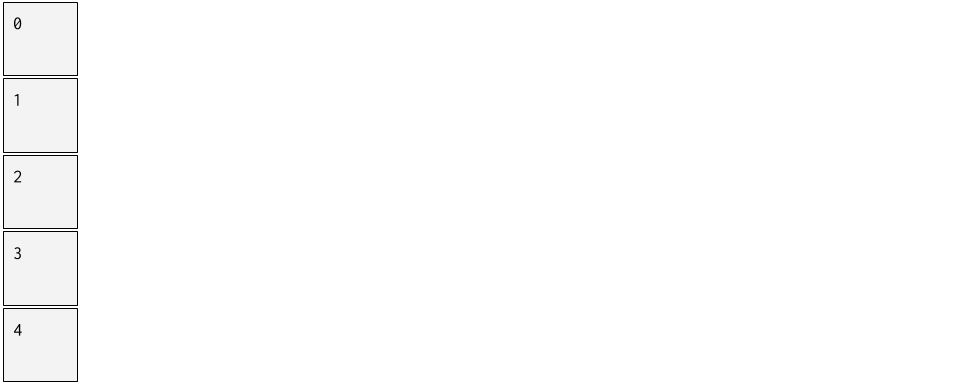
\includegraphics[width=\textwidth]{hashmap}
\fi

\begin{solution}
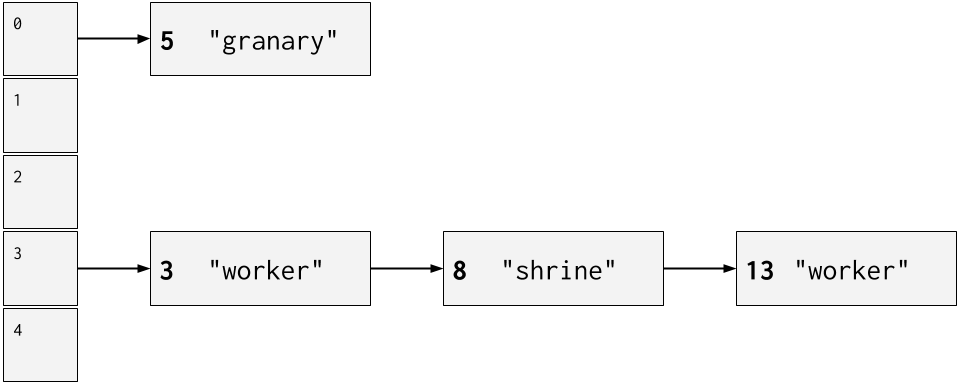
\includegraphics[width=\textwidth]{hashmap-sol}
\lstinline$"worker"$ replaces \lstinline$"monument"$ as their keys are the
same. Each \lstinline$put$ must iterate through the entire external chain to
ensure that a key-update is not necessary.
\end{solution}

\begin{parts}
\part What happens if you resize the array, double its length, and put everything back in?
\begin{solution}[1.0in]
The value of "shrine" and "granary" will move. Specifically, the new length of the array is 10. A key of 8 will force "shrine" to be placed in the 8th index. A key of 5 will move "granary" to the 5th index. Everything else will remain the same.
\end{solution}
\end{parts}
\end{blocksection}
